%=============================================================================
% Thesis Template in LaTex
%
% File:  05-Resultate.tex -- Resultate
% Author(s): Cyrano Golliez <golliezc@student.ethz.ch>
%
% Creation:  27 Jan 2014
% Time-stamp: <Tue 2013-08-13 20:14 juergen>
%
% Copyright (c) 2014 Infrastructure Management Group (IMG)
%               http://ibi.ethz.ch
%
% More information on LaTeX: http://www.latex-project.org/
%=============================================================================

\chapter{Resultate}
\label{chap:Resultate}

Um die Verkehrssituation am Bahnübergang Brunnenstrasse nachhaltig zu verbessern, bedarf es einer optimalen Variante, die durch den Vergleich der gemäss Abschnitt \ref{subsec:BerechnungRisiken} berechneten Risiken der Varianten bestimmt wird. 
Nachfolgend dargestellt sind die Resultate der Risikoberechnung sowie der Risikovergleich und für die verschiedenen Sensitivitätsanalysen die als optimal bestimmte Variante. 

\begin{figure}[h!]
  \centering
  \subfloat[][]{\label{img:RisikoVar-Z0)}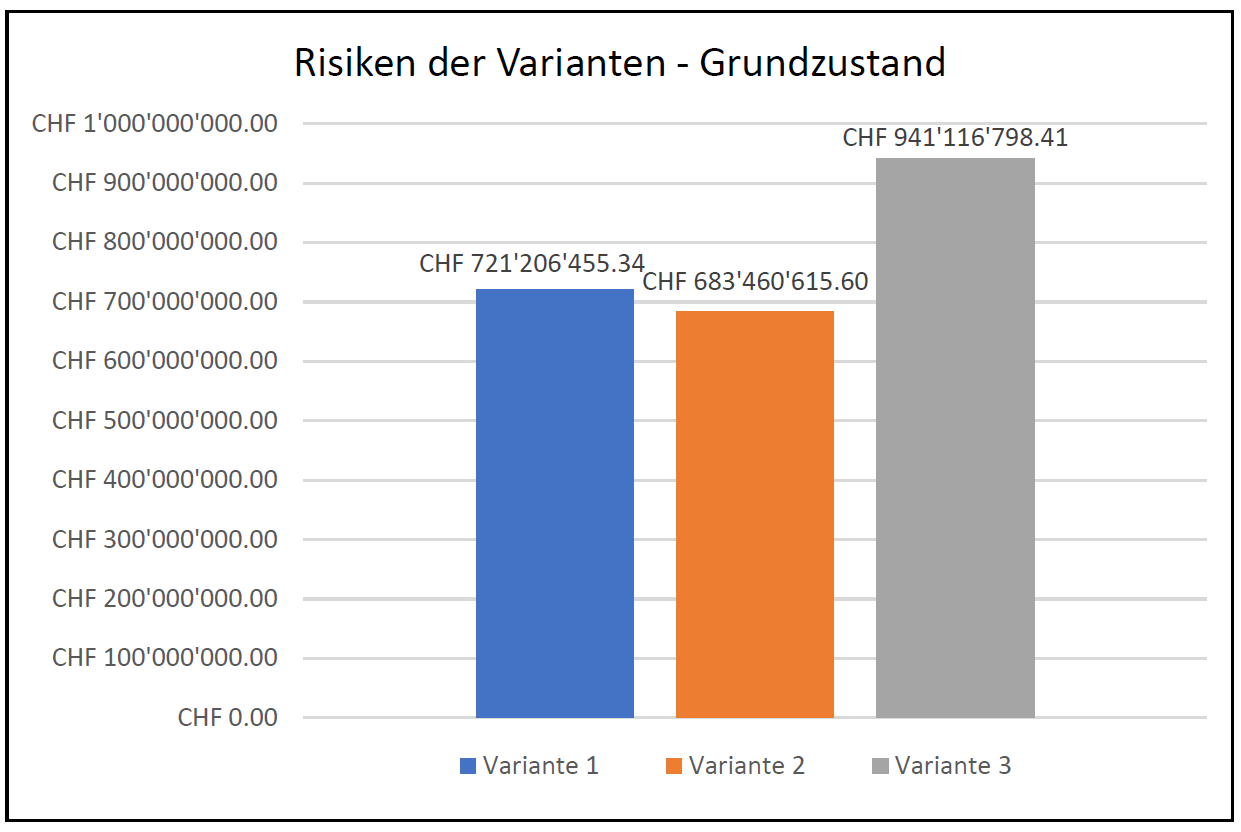
\includegraphics[width=.5\textwidth]{./figures/f-05-02-RisikenVarianteZ0}}
  \hfill
  \subfloat[][]{\label{img:VariantenwahlZ0)}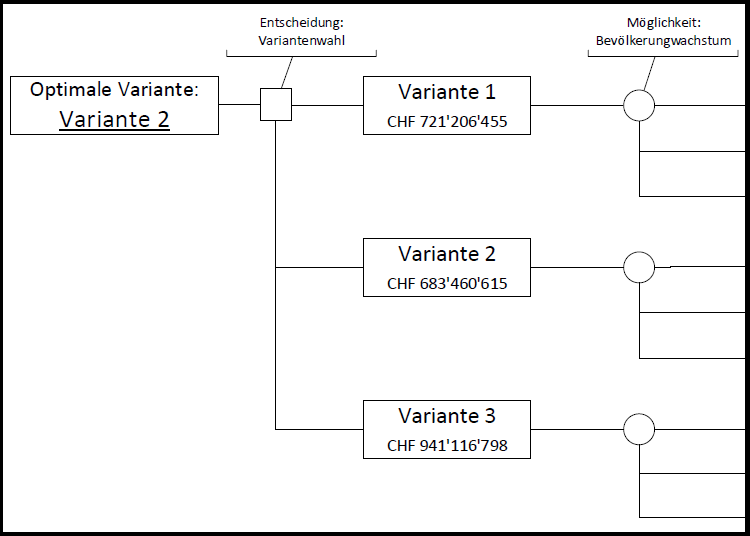
\includegraphics[width=.5\textwidth]{./figures/f-05-01-Variantenwahl}}
\caption[Risikovergleich Grundzustand]{Risikovergleich und Entscheidungsprozess im Grundzustand}
  \label{fig:Z0}
\end{figure}

\paragraph{Grundzustand}

Wie in der Abbildung \ref{img:Z0} ersichtlich, beträgt das Risiko der Variante 1 im Grundzustand 721'206'455 CHF, das Risiko der Variante 2 683'460'615 CHF und das Risiko der Variante 3 941'116'798 CHF. Das Risiko der Variante 2 ist somit um 37'745'840 CHF geringer als das Risiko der Variante 1 und um 257'656'183 CHF kleiner als das Risiko der Variante 3. Die Differenz der Risiken der Varianten 1 und 3 beträgt 219'910'343 CHF. \\
Die Variante mit dem geringsten Risiko im Grundzustand ist demnach Variante 2 und ist dementsprechend die optimale Variante, wie in Abbildung \ref{fig:Z0} dargestellt.

\paragraph{Parameterauswahl 1, 2 und 3}

Die nachfolgende Abbildung \ref{img:RisikovergleichVarianten123} stellt die Risiken der Varianten für die Parameterauswahl 1, 2 und 3 dar. Es ist klar ersichtlich, dass sich in der Parameterauswahl 1, 2 und 3 keine Veränderung ergibt und weiterhin die Variante 2 die optimale Lösung darstellt. Aus diesem Grund verzichte ich auf die ausführliche Darstellung und verweise auf das Kapitel \ref{chap:Diskussion} in dem ich die verschiedenen Parameterauswahlen ausführlich vergleiche und diskutiere.

\begin{figure}[h!]
	\centering
	\includegraphics[width=\textwidth]{figures/f-05-00-01-RisikenVergleichZustände1-3}
	\caption[Risikovergleich der Parameterauswahl 1, 2 und 3]{Risikovergleich der Varianten - Parameterauswahl 1, 2 und 3}
	\label{img:RisikovergleichVarianten123}
\end{figure}

\paragraph{Parameterauswahl 4}

Für die Parameterauswahl 4 beträgt das Risiko der Variante 1 wie im Grundzustand 721'206'455 CHF. Das Risiko der Variante 2 beträgt 683'460'616 CHF und das Risiko der Variante 3 ist mit 683'422'520 CHF deutlich niedriger als im Grundzustand. In Abbildung \ref{img:Z4-V2/V3)} wird der Vergleich der Varianten 2 und 3 gezeigt, wo man erkennen kann, dass die Differenz der berechneten Risiken 38'095 CHF beträgt.

Aufgrund der berechneten Risiken für die Parameterauswahl 4 und unter den getroffenen Annahmen, ist die Variante 3 die optimale Lösung zur bedarfsgerechten Verbesserung der Verkehrssituation am Bahnübergang. Eine Diskussion dieser Lösung folgt im Kapitel \ref{chap:Diskussion}.

\begin{figure}[h!]
  \centering
  \subfloat[][]{\label{img:RisikenZ4)}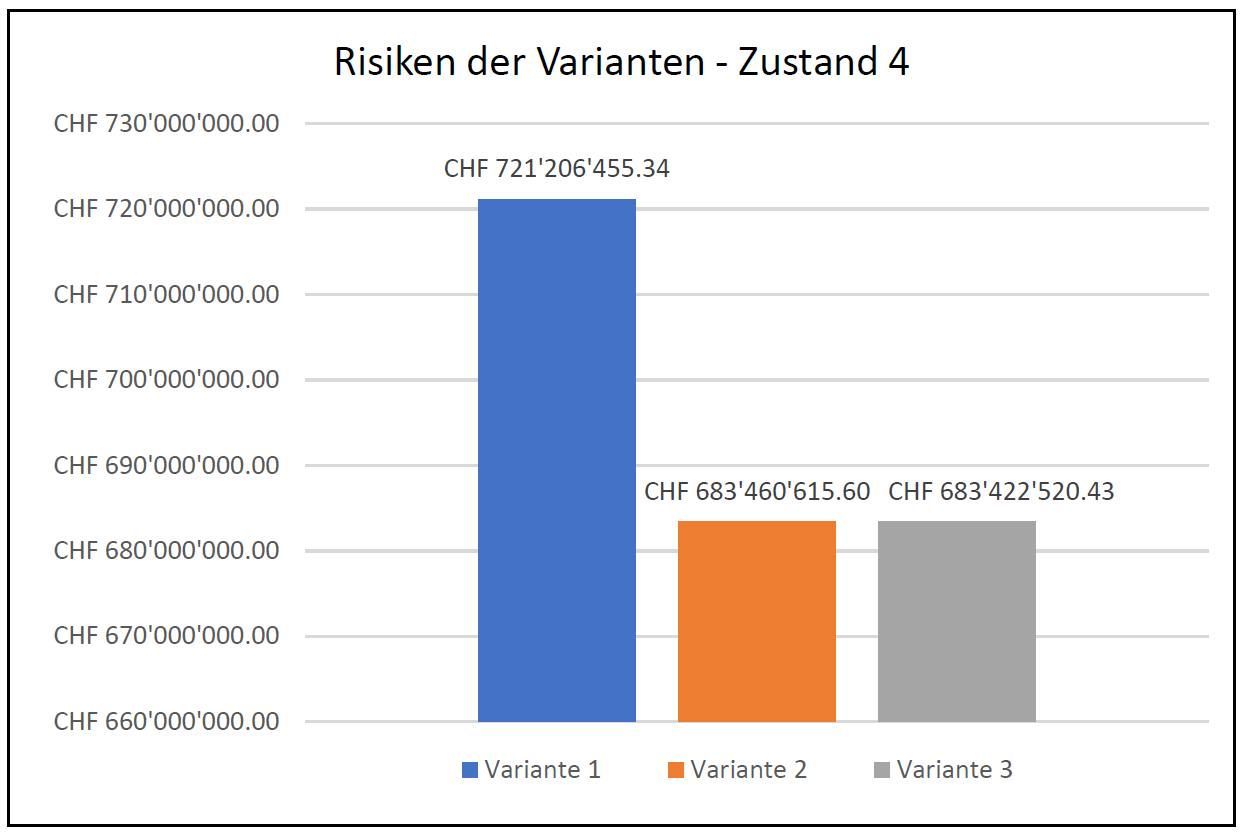
\includegraphics[width=.5\textwidth]{./figures/f-05-05-RisikenVarianteZ4}}
  \hfill
  \subfloat[][]{\label{img:Z4-V2/V3)}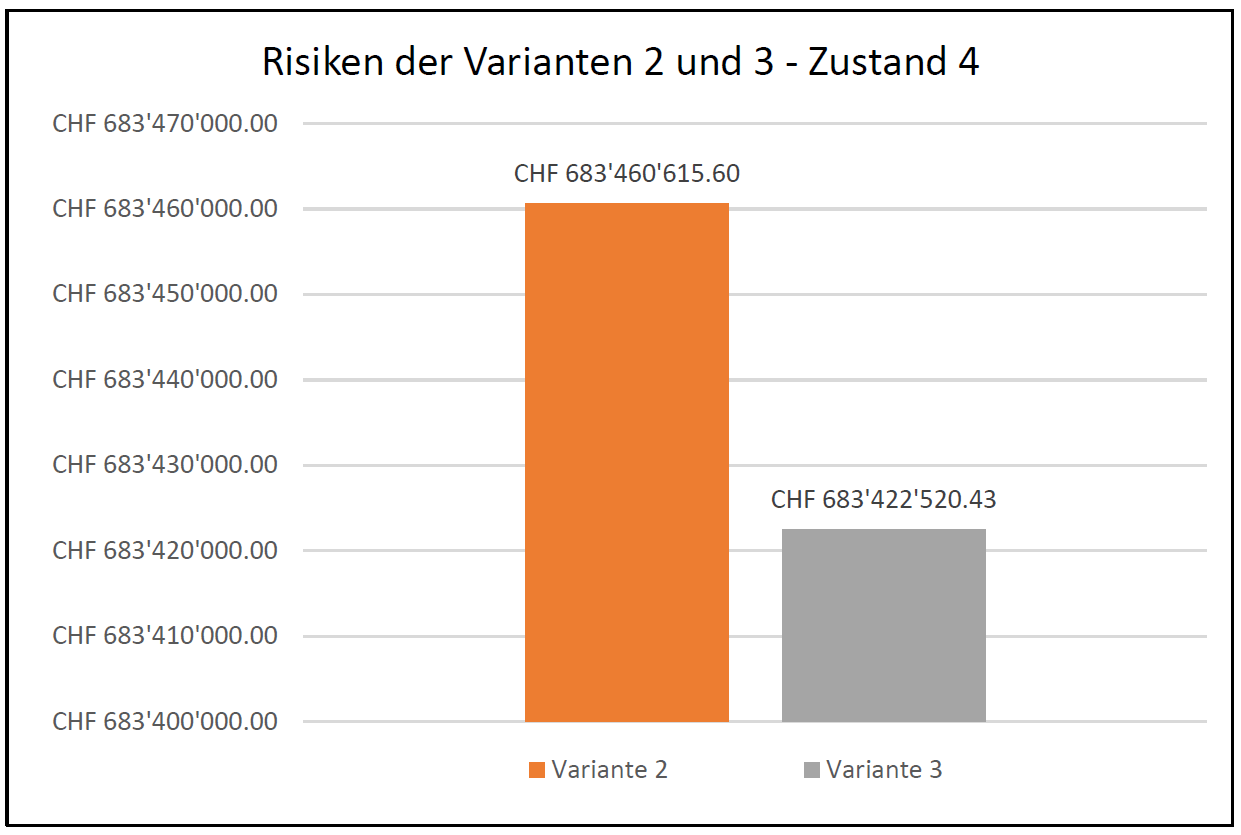
\includegraphics[width=.5\textwidth]{./figures/f-05-06-RisikenVariante-2und3-Z4}}
\caption[Risikovergleich Parameterauswahl 4]{Risikovergleich für die Parameterauswahl 4}
  \label{fig:Parameter4}
\end{figure}



% ===========================================================================
% EOF
%

%%% Local Variables:
%%% mode: latex
%%% TeX-master: "../main"
%%% End:
